\begin{comment}
\title{parslTestbookQMCblog}
\author{Dr. Sou-Cheng Choi, Illinois Tech and SouLab, Joshua Jay Herman (QMC Development Team)}
\date{September 2025}

\maketitle
Accelerating QMCpy Notebook Tests with Parsl
\end{comment}

\subsection{Introduction}

 This blog provides a summary of the speedup of notebook regression testing presented in our talk at ParslFest \cite{parslfest2025} 
 and highlights the subsequent directions of the work. Regression testing of notebooks for QMCPy \cite{QMCPy2020a} is massively parallel and resource-intensive.

\subsection{Methodology}

 Choosing Testbook \cite{testbook2021} was primarily motivated by the usability of actually writing a test (one that would even execute the notebook itself). It also fits well with our tests in a separate directory, where we have already implemented other tests without requiring execution of the full notebooks for clarity. Then we made a test harness that we could also have Parsl \cite{parsl2019} execute our testbook unittests since it is embarrassingly parallel.

\subsection{Results}

To determine a baseline speedup with a subset of notebooks, we saw a speedup. 
After increasing our test coverage, which expanded our work to look for syntax errors in more notebooks, we now see a 4.4x speedup, which is consistent with our expectations, as shown in Figure~\ref{fig:parsl_speedup}. 

\begin{figure}[htbp]
    \centering
    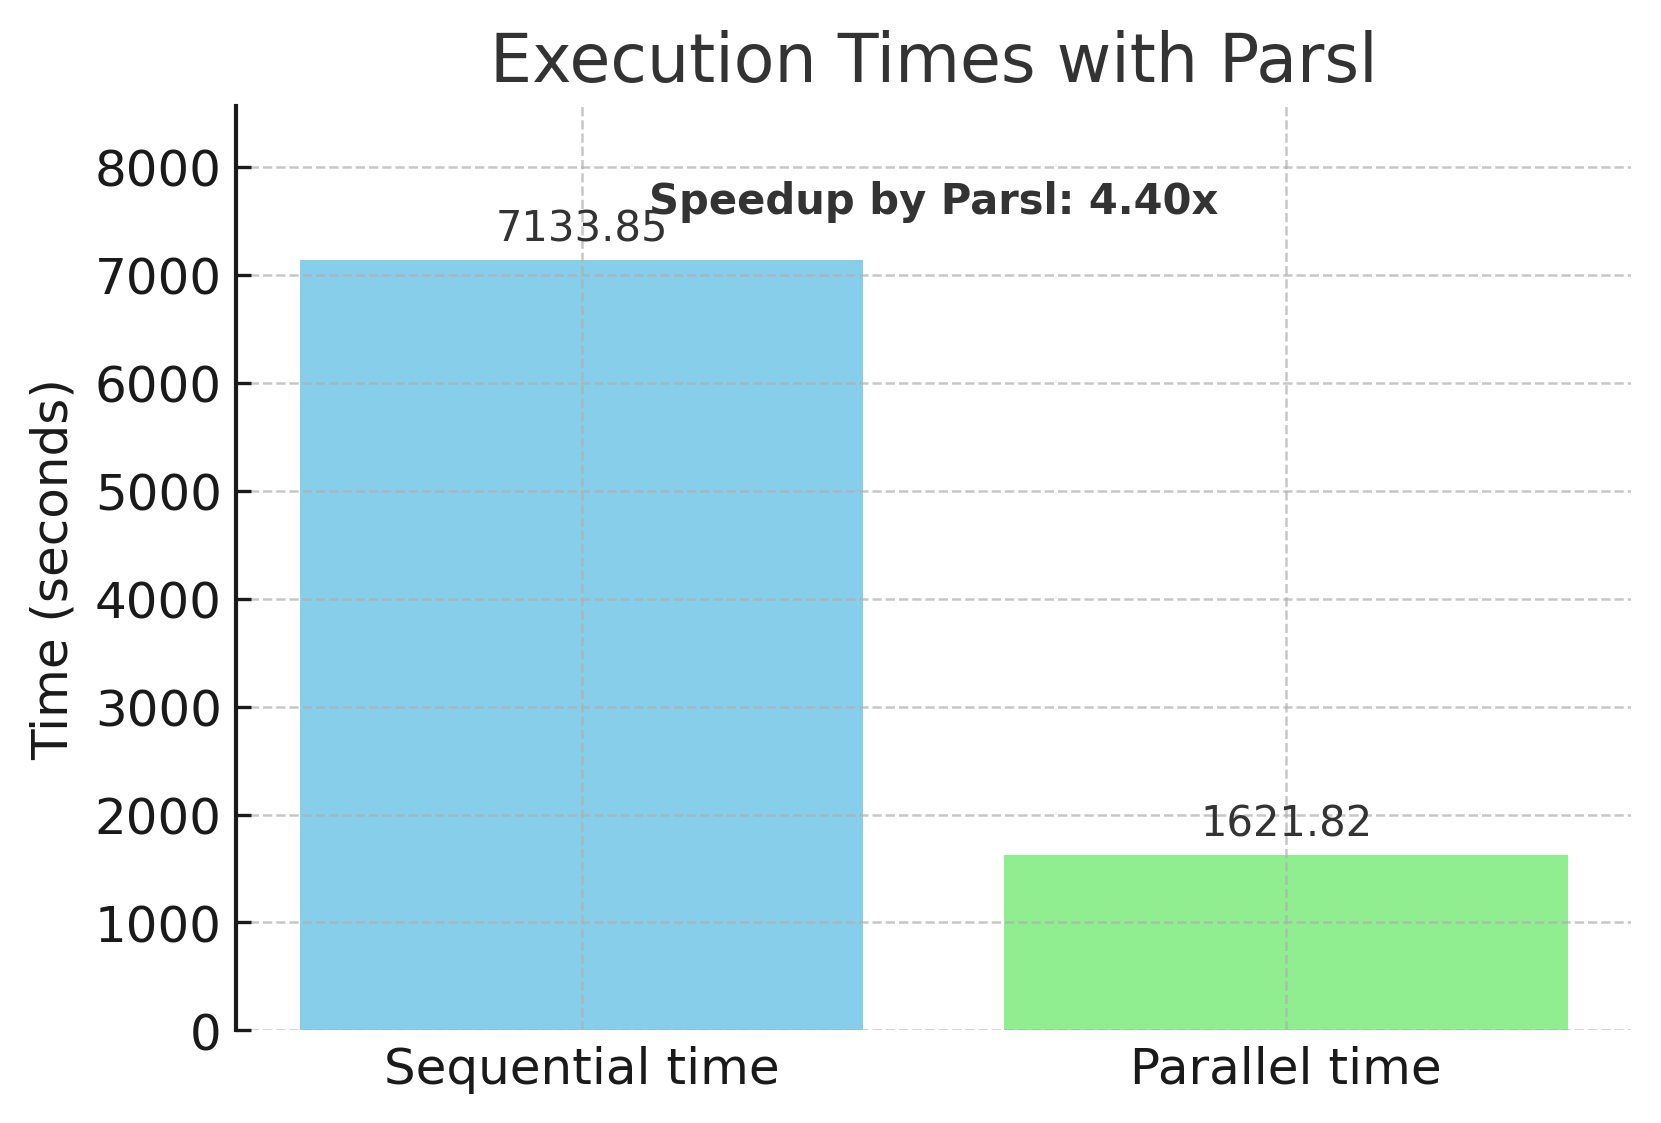
\includegraphics[width=.7\textwidth]{booktests/parsl_speedup_chart_no_x_lines.png}
    \caption{Parallel testing speedup using Parsl against sequential execution of tests.}
    \label{fig:parsl_speedup}
\end{figure}

\scnote{Add details about architecture where the speedup were observed.}

\subsection{Further Work}

Due to the above results, this points to the fact that we should extend our testing to doctest and pytests in Parsl.

Now, since many people have multi-core processors, we can make our individuals more productive so that our tests can show that no regressions have been introduced faster.

Last but not least of the feedback on the presentation of this work to the Parsl group would be that the system is very general. This implies that a distributed test system could be interesting for Parsl users to distribute their own test workloads. 
Also, extending our work to not just test Jupyter notebooks, but also Python-based doctests, adding new testing such as Behavior-Driven Development using Cucumber \cite{cucumber2025}, unit testing using pytest and/or unittest.

\scnote{How to apply ``Cucumber tests for Behavior-Driven Development'' in QMCPy?}

\scnote{Add a link to the presentation slides and notebooks}

\scnote{add make testbook and add to readme on running juypter notebook tests}

\scnote{workflow fixing to github actions ask IIT person presentation}

\scnote{alexander culler ( german) lookup nvidia mental images , art owen}


